% abtex2-modelo-artigo.tex, v-1.9.2 laurocesar
% Copyright 2012-2014 by abnTeX2 group at http://abntex2.googlecode.com/ 
%

% ------------------------------------------------------------------------
% ------------------------------------------------------------------------
% abnTeX2: Modelo de Artigo Acadêmico em conformidade com
% ABNT NBR 6022:2003: Informação e documentação - Artigo em publicação 
% periódica científica impressa - Apresentação
% ------------------------------------------------------------------------
% ------------------------------------------------------------------------

\documentclass[
% -- opções da classe memoir --
article,			% indica que é um artigo acadêmico
11pt,				% tamanho da fonte
oneside,			% para impressão apenas no verso. Oposto a twoside
a4paper,			% tamanho do papel. 
% -- opções da classe abntex2 --
%chapter=TITLE,		% títulos de capítulos convertidos em letras maiúsculas
%section=TITLE,		% títulos de seções convertidos em letras maiúsculas
%subsection=TITLE,	% títulos de subseções convertidos em letras maiúsculas
%subsubsection=TITLE % títulos de subsubseções convertidos em letras maiúsculas
% -- opções do pacote babel --
english,			% idioma adicional para hifenização
brazil,				% o último idioma é o principal do documento
sumario=tradicional
]{abntex2}


% ---
% PACOTES
% ---

% ---
% Pacotes fundamentais 
% ---
\usepackage{lmodern}			% Usa a fonte Latin Modern
\usepackage[T1]{fontenc}		% Selecao de codigos de fonte.
\usepackage[utf8]{inputenc}		% Codificacao do documento (conversão automática dos acentos)
\usepackage{indentfirst}		% Indenta o primeiro parágrafo de cada seção.
\usepackage{nomencl} 			% Lista de simbolos
\usepackage{color}				% Controle das cores
\usepackage{graphicx}			% Inclusão de gráficos
\usepackage{float}
\usepackage{microtype} 			% para melhorias de justificação

% ---

% ---
% Pacotes adicionais, usados apenas no âmbito do Modelo Canônico do abnteX2
% ---
\usepackage{lipsum}				% para geração de dummy text
% ---

% ---
% Pacotes de citações
% ---
\usepackage[brazilian,hyperpageref]{backref}	 % Paginas com as citações na bibl
\usepackage[alf]{abntex2cite}	% Citações padrão ABNT
% ---

% ---
% Informações de dados para CAPA e FOLHA DE ROSTO
% ---
\titulo{Atividade VIII}
\autor{ Rafael Gonçalves de Oliveira Viana}
\local{Brasil}
\data{2017}
% ---

% ---
% Configurações de aparência do PDF final

% alterando o aspecto da cor azul
\definecolor{blue}{RGB}{41,5,195}

% informações do PDF
\makeatletter
\hypersetup{
	%pagebackref=true,
	pdftitle={\@title}, 
	pdfauthor={\@author},
	pdfsubject={Artigo},
	pdfcreator={LaTeX with abnTeX2},
	pdfkeywords={abnt}{latex}{abntex}{abntex2}{atigo científico}, 
	colorlinks=true,       		% false: boxed links; true: colored links
	linkcolor=blue,          	% color of internal links
	citecolor=blue,        		% color of links to bibliography
	filecolor=magenta,      		% color of file links
	urlcolor=blue,
	bookmarksdepth=4
}
\makeatother
% --- 

% ---
% compila o indice
% ---
\makeindex
% ---

% ---
% Altera as margens padrões
% ---
\setlrmarginsandblock{3cm}{3cm}{*}
\setulmarginsandblock{3cm}{3cm}{*}
\checkandfixthelayout
% ---

% --- 
% Espaçamentos entre linhas e parágrafos 
% --- 

% O tamanho do parágrafo é dado por:
\setlength{\parindent}{1.3cm}

% Controle do espaçamento entre um parágrafo e outro:
\setlength{\parskip}{0.2cm}  % tente também \onelineskip

% Espaçamento simples
\SingleSpacing

% ----
% Início do documento
% ----
\begin{document}
	
	% Retira espaço extra obsoleto entre as frases.
	\frenchspacing 
	
	% ----------------------------------------------------------
	% ELEMENTOS PRÉ-TEXTUAIS
	% ----------------------------------------------------------
	
	%---
	%
	% Se desejar escrever o artigo em duas colunas, descomente a linha abaixo
	% e a linha com o texto ``FIM DE ARTIGO EM DUAS COLUNAS''.
	% \twocolumn[    		% INICIO DE ARTIGO EM DUAS COLUNAS
	%
	%---
	% página de titulo
	\maketitle
	\begin{enumerate}
	
	
		\item Create or replace trigger t\_io\_vPessoas
				\begin{verbatim}
		
		create or replace trigger t_io_vPessoas
		instead of insert
		on vPessoas
		declare v_cod_instrutor number; v_matricula_aluno number;
		begin
		select max(cod_instrutor)+1 into v_cod_instrutor from instrutores;
		select max(matricula)+1 into v_matricula_aluno from alunos;
		if :new.tipo = 'a' then --aluno!
		insert into alunos (matricula, nome_aluno) values
		(v_matricula_aluno, :new.nome);
		else
		insert into instrutores (cod_instrutor, nome_instrutor)
		values (v_cod_instrutor, :new.nome);
		end if;
		end;
			 \end{verbatim}
			 \begin{center}
			 	\begin{figure}[H]
			 		\centering
			 		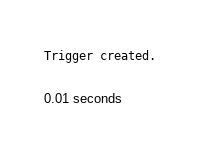
\includegraphics[scale=0.5]{./imagens/22.png}
			 		\caption{	create or replace trigger .}
			 		\label{rota-1}
			 	\end{figure}
			 \end{center}
					
			insert into vPessoas (nome, tipo) values ('Aluno', 'a');

					\begin{center}
					\begin{figure}[H]
						\centering
						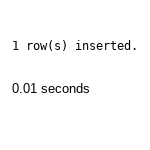
\includegraphics[scale=0.5]{./imagens/23.png}
						\caption{insert into vPessoas  .}
						\label{rota-1}
					\end{figure}
				\end{center}

					
			insert into vPessoas (nome, tipo) values ('Instrutor', 'i');

					\begin{center}
					\begin{figure}[H]
						\centering
						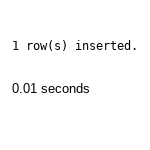
\includegraphics[scale=0.5]{./imagens/23.png}
						\caption{insert into vPessoas  .}
						\label{rota-1}
					\end{figure}
				\end{center}
	
			
			select * from instrutores where nome\_instrutor = 'Instrutor'
			
				 \begin{center}
					\begin{figure}[H]
						\centering
						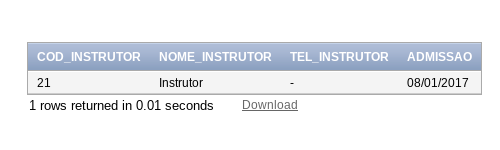
\includegraphics[scale=0.5]{./imagens/25.png}
						\caption{	select * from instrutores}
						\label{rota-1}
					\end{figure}
				\end{center}
			
			select * from alunos where nome\_aluno = 'Aluno'
				 \begin{center}
					\begin{figure}[H]
						\centering
						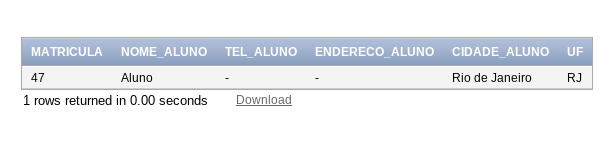
\includegraphics[scale=0.5]{./imagens/26.png}
						\caption{	select * from alunos.}
						\label{rota-1}
					\end{figure}
		    	\end{center}
			drop view vPessoas;
				 \begin{center}
					\begin{figure}[H]
						\centering
						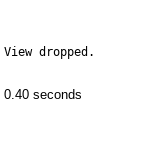
\includegraphics[scale=0.5]{./imagens/28.png}
						\caption{	drop view vPessoas.}
						\label{rota-1}
					\end{figure}
				\end{center}
			drop trigger t\_io\_vPessoas;
			
			\begin{center}
				\begin{figure}[H]
					\centering
					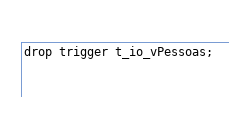
\includegraphics[scale=0.5]{./imagens/29.png}
					\caption{drop trigger t\_io\_vPessoas;
						s.}
					\label{rota-1}
				\end{figure}
			\end{center}
						\item create or replace trigger t\_aft\_upd\_row\_AumentaPrecos
					\begin{verbatim}
					create or replace trigger t_aft_upd_row_AumentaPrecos
					after update
					on cursos
					for each row
					begin
					if :new.preco > 1200 then
					raise_application_error(-20500, 'Tentativa
					exagerada de aumento!');
					end if;
					end;
					\end{verbatim}
					\begin{center}
						\begin{figure}[H]
							\centering
							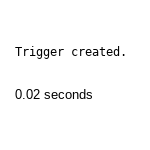
\includegraphics[scale=0.5]{./imagens/30.png}
							\caption{	create or replace trigger .}
							\label{rota-1}
						\end{figure}
					\end{center}
					
					
							\item create sequence
				\begin{verbatim}
			create sequence gera_matr_aluno
			start with 40 increment by 1 maxvalue 1000
			nocycle;
				\end{verbatim}
				\begin{center}
					\begin{figure}[H]
						\centering
						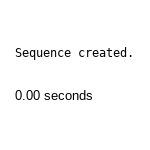
\includegraphics[scale=0.5]{./imagens/31.png}
						\caption{	create sequence  .}
						\label{rota-1}
					\end{figure}
				\end{center}
								\item 	create or replace trigger t\_bef\_ins\_row\_InsereAluno
			\begin{verbatim}
		create or replace trigger t_bef_ins_row_InsereAluno
		before insert
		on alunos
		for each row
		declare
		nova_matricula number;
		begin
		select Gera_Matr_aluno.Nextval
		into nova_matricula from dual;
		:new.matricula := nova_matricula;
		end;
			\end{verbatim}
			\begin{center}
				\begin{figure}[H]
					\centering
					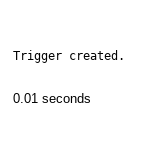
\includegraphics[scale=0.5]{./imagens/32.png}
					\caption{	create or replace trigger .}
					\label{rota-1}
				\end{figure}
			\end{center}
							\begin{verbatim}
				create or replace trigger
				t_bef_upd_stm_Registro
				before update
				on cursos
				Begin
				update Tab_Auditoria
				set atualizacoes = atualizacoes + 1;
				end;
					\end{verbatim}
					\begin{center}
						\begin{figure}[H]
							\centering
							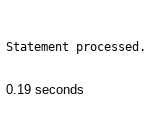
\includegraphics[scale=0.5]{./imagens/33.png}
							\caption{	create or replace trigger .}
							\label{rota-1}
						\end{figure}
					\end{center}
									\begin{verbatim}
				create or replace trigger
				t_bef_del_row_LimpaHist
				before delete
				on turmas
				for each row
				begin
				delete historico
				where cod_turma = :old.cod_turma;
				end;
					\end{verbatim}
					\begin{center}
						\begin{figure}[H]
							\centering
							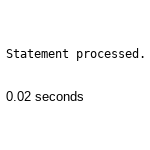
\includegraphics[scale=0.5]{./imagens/34.png}
							\caption{	create or replace trigger .}
							\label{rota-1}
						\end{figure}
					\end{center}
											\begin{verbatim}
			create or replace trigger t_bef_updIns_stm_MultHist
			before insert or update
			on historico
			declare
			v_hoje number;
			v_agora number;
			begin
			v_hoje := to_number(to_char(sysdate,'dd'));
			v_agora := to_number(to_char(sysdate,'hh24mi'));
			if inserting then
			if v_agora > 1830 then
			raise_application_error(-20600, 'Hora proibida para
			inserções');
			end if;
			else
			if v_hoje = 1 then
			raise_application_error(-20700, 'Dia proibido para
			atualizações');
			end if;
			end if;
			end;
				\end{verbatim}
				\begin{center}
					\begin{figure}[H]
						\centering
						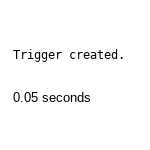
\includegraphics[scale=0.5]{./imagens/35.png}
						\caption{	create or replace trigger .}
						\label{rota-1}
					\end{figure}
				\end{center}
			
		
			
														\begin{verbatim}
		Set serveroutput on; //variável de ambiente.
		declare saida varchar2(40);
		begin
		saida:=exclui_instrutores_cursor_imp;
		dbms_output.put_line('Saida: '||saida);
		end;
			\end{verbatim}
				\begin{center}
				\begin{figure}[H]
					\centering
					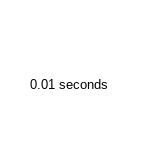
\includegraphics[scale=0.5]{./imagens/37.png}
					\caption{	Set serveroutput on .}
					\label{rota-1}
				\end{figure}
			\end{center}
		

	\end{enumerate}				
			
\end{document}
